%File: main.tex
\documentclass[letterpaper]{article}
\usepackage{aaai2026}
\usepackage{times}
\usepackage{helvet}
\usepackage{courier}
\usepackage[hyphens]{url}
\usepackage{graphicx}
\usepackage{natbib}
\usepackage{caption}
\usepackage{booktabs}
\usepackage{amsmath}
\usepackage{multirow}
\frenchspacing
\setlength{\pdfpagewidth}{8.5in}
\setlength{\pdfpageheight}{11in}
\setcounter{secnumdepth}{1}
\pdfinfo{/TemplateVersion (2026.1)}
\nocopyright

\title{Five Million Parameters on CIFAR-10: What Worked, What Did Not, and an Unexplained Test Gap}

\author{
  Philip Vetsas\textsuperscript{\rm 1},
  Rahim Askarov\textsuperscript{\rm 1}
}

\affiliations{
  \textsuperscript{\rm 1}NYU Tandon School of Engineering, CS-GY 6923 Deep Learning, Fall 2026\\
  Team P.R. \quad \{pmv264, ra3716\}@nyu.edu
}

\begin{document}
\maketitle

\begin{abstract}
We train a 4.88M-parameter ResNet from scratch on CIFAR-10 under a hard 5M
parameter budget and a hidden evaluation set. Our best recipe combines a long
cosine schedule, SAM, EMA, and knowledge distillation from three auxiliary
teachers, reaching 97.84\% clean validation accuracy (97.92\% with 10-view TTA).
The team's selected submissions scored 0.911 and 0.904 on the public leaderboard;
the private score was 0.880, placing 13th. The roughly ten-point gap between
validation and private accuracy is unexplained, and we report it as observed
rather than optimizing against it. We focus on measured training experiments:
long schedules and KD give the largest gains, architecture changes inside the 5M
budget give small ones, and a long list of plausible techniques did not work.
One-view AugMix was clean-neutral at 300 epochs and improved corrupted and
photometric proxies, but it was not shipped because its KD confirmation finished
after submission selection; an AugMix+JSD variant traded clean accuracy for blur
robustness and was rejected. We document the failed techniques with paired
statistics and validation curves.
\end{abstract}

\section{Introduction}

CIFAR-10 is a small-data benchmark that modern architectures have largely
saturated: with tens of millions of parameters and long schedules, test accuracy
above 99\% is routine. The problem changes when the model must be trained from
scratch under a hard budget of five million trainable parameters, and when the
evaluation set is hidden and may not match the training distribution. Both
constraints were active in this competition. The first forces careful
architecture and optimization choices; the second makes validation accuracy an
imperfect guide and turns the leaderboard into a noisy, partially observed
signal.

We approached the problem as a two-track collaboration. One track pushed clean
accuracy through architecture search, long schedules, and knowledge distillation
(KD) from large teachers trained on the same data. The other track studied
robustness: it characterized the only unlabeled images available to us, built
corrupted and photometric proxy validation sets from the training split, and ran
controlled augmentation ablations. The two tracks shared one codebase, one fixed
5,000-image holdout, and one set of conventions, so every number in this paper is
directly comparable.

The main result is a 4.88M-parameter student that reaches 97.84\% clean
validation accuracy and 97.92\% with 10-view test-time augmentation (TTA). The team's selected
submissions scored 0.911 and 0.904 on the public leaderboard; the team's private
score was 0.880, placing 13th. The roughly ten-point gap between
our best holdout number and the private score is the central unsolved problem of
the project.

An important caveat shapes how we interpret that gap. The 2,000 unlabeled images
distributed with the starter data, which we analyzed at length, were not the
images used for the final leaderboard. Our photometric statistics, nearest-
neighbor tests, and visual comparisons therefore describe that released sample,
not the final test set. They motivated the robustness experiments and gave us a
useful analysis pipeline, but they cannot explain the final score. We report them
as exploratory evidence and explicitly separate them from the leaderboard
outcome. The only direct evidence of a distribution difference is the gap between
validation and leaderboard accuracy itself.

This paper makes four contributions.
\begin{itemize}
\item A strong, reproducible 4.88M-parameter recipe: long cosine training, SAM,
EMA, TrivialAugment, Cutout, mixup/CutMix, and three-teacher KD. It improves a
plain baseline from 94.76\% to 97.84\% validation (97.92\% with TTA) and yields
the team's 0.911 public / 0.880 private submissions.
\item A controlled account of which ingredients mattered. Long schedules and KD
gave the largest gains; architecture changes within the 5M budget gave small ones;
several plausible tricks did not pay off.
\item A clean-neutral augmentation result: AugMix leaves clean accuracy unchanged
but improves a composite corruption proxy by 2.2pp and a photographic-jitter proxy
by 1.9pp, replicated across seeds and surviving distillation.
\item A negative-results and uncertainty report. We document failed techniques
with paired statistics and validation curves, and we separate proxy evidence from
evidence about the hidden test set.
\end{itemize}

Section~\ref{sec:related} reviews related work. Section~\ref{sec:setup} defines
the protocol. Section~\ref{sec:method} describes the architectures, training
recipe, KD variants, augmentation policies, and proxy analyses.
Section~\ref{sec:results} presents accuracy and robustness results.
Section~\ref{sec:negative} collects the techniques that underperformed.
Section~\ref{sec:discussion} discusses the gap and limitations;
Section~\ref{sec:conclusion} concludes.

\section{Setup and Protocol}
\label{sec:setup}

\paragraph{Data and splits.}
We use the 50,000 labeled CIFAR-10 training images (10 classes, $32\times32$
RGB). A fixed stratified 5,000-image holdout (split seed 0) is used by every
student and every teacher; the remaining 45,000 images are used for training.
Teachers and students must hold out the same images, otherwise teacher
predictions on the holdout leak into the student through the soft targets. The
final full-data models are retrained on all 50,000 images once the recipe is
fixed. No external data and no pretrained weights are used.

\paragraph{Evaluation.}
The competition metric is top-1 accuracy. The public and private leaderboards each
use 1,000 hidden images, so a public score near 90\% has a standard error of about
1.1 percentage points; we do not select models by small public differences. Unless
stated otherwise, validation numbers use EMA weights. We report raw, EMA, flip
TTA (average of the image and its horizontal mirror), and 10-view TTA. The latter,
which we call \emph{5-crop} to match the competition codebase, averages the
softmax over a center view and four $\pm2$-pixel shifts, each with and without a
horizontal flip.

\paragraph{Paired statistics.}
Model comparisons use McNemar's exact test on per-image correctness over the same
5,000 holdout images. We report the discordant counts and two-sided binomial
$p$-values. The seed-to-seed spread on this holdout is about 0.2pp on clean data
and 0.4pp on the composite proxy, so differences of that size are treated as
noise.

\paragraph{Rules.}
The official overview asks for a modified ResNet with at most 5M trainable
parameters, trained from scratch on the permitted CIFAR-10 training data, with no
pretrained weights or external datasets. The evaluation images may not be
labeled, used for training, or used for model selection. We apply the budget to
the submitted network; the teachers are auxiliary models trained from scratch on
the same 50,000 images and are not part of the submitted inference system. The
team submits a single network per submission.

\paragraph{Validation proxies.}
We build shifted validation sets from the 5,000 holdout images only. The
corruptions are Gaussian noise ($\sigma=0.05,0.10$), Gaussian blur (radius 1.0,
2.0), JPEG compression (quality 30), contrast scaling (0.7, 1.3), color
saturation (1.3), and a composite \emph{combo} (contrast 1.15, brightness 1.05,
blur 0.5, Gaussian noise $\sigma=0.02$, JPEG 75). The photographic proxies apply
per-image brightness/contrast/saturation scaling plus a small zoom and rotation:
\emph{mild} uses $\pm8\%$ brightness/contrast, $\pm12\%$ saturation, zoom 1.05 and
$\pm3^\circ$; \emph{strong} uses $\pm20\%$, $\pm30\%$, zoom 1.15 and $\pm6^\circ$.
These are label-free stress tests built from training images, not models of the
final test set.

\paragraph{Compute.}
Main runs used NYU HPC A100 nodes; ablations used A10-class cloud GPUs and a local
RTX 2070. A 4.9M student takes about 19--21s per epoch on an A10-class GPU;
three-teacher distillation takes about 59s per epoch. The longest runs (1,200
epochs on all 50k images) take several hours.

\section{Methods}
\label{sec:method}

\subsection{Architectures}

\paragraph{Students.}
Our student family is a pre-activation bottleneck ResNet. A $3\times3$ stem
produces the first stage's channels and keeps the $32\times32$ resolution; three
stages then use 3/5/3 or 2/3/3 basic blocks, with the first block of stages 2 and
3 applying stride 2. Each block computes
$\mathrm{ReLU}(F(x)+S(x))$, where $F$ is conv--BN--ReLU--conv--BN, the last BN is
zero-initialized so the block starts as an identity, and $S$ is an identity or a
$1\times1$ conv--BN shortcut when the shape changes. A global average pool and a
linear layer produce the logits. The two selected presets are
\texttt{r3\_64\_3-5-3} (64/128/256 channels, 3/5/3 blocks, 4.92M parameters) and
\texttt{r3\_80\_2-3-3} (80/160/256, 2/3/3, 4.88M). A 300-epoch sweep also
evaluated \texttt{r3\_96\_2-2-2} (4.90M), \texttt{r4\_64\_3-3-2-1} (4.89M), and
\texttt{r3\_40\_8-8-8} (4.72M).

\paragraph{Teachers.}
We use two WRN-28-10 teachers \citep{zagoruyko2016wide} (36.5M parameters each,
seeds 0 and 1) and one PyramidNet-110-270 teacher \citep{han2017deep} with
ShakeDrop (28.5M, seed 2). Teachers are trained for 400
epochs with the same augmentation recipe but a different seed each; teacher size
is not constrained by the 5M budget because only the student is submitted. The
teacher pool reaches 98.14\% holdout accuracy (WRN seeds 0+1); the individual
teachers reach 98.06, 98.12, and 97.64.

\subsection{Training Recipe}

All students use SGD with Nesterov momentum 0.9, batch size 128, base learning
rate 0.1, weight decay $5\times10^{-4}$ (not applied to BN affine parameters or
biases), a 5-epoch linear warmup followed by cosine decay to zero, and bf16 autocast. The default augmentation is random
crop with 4-pixel padding plus horizontal flip, TrivialAugment
\citep{muller2021trivialaugment}, Cutout 16 \citep{devries2017cutout}, and per-batch
mixup \citep{zhang2018mixup} ($\alpha=0.2$) or CutMix \citep{yun2019cutmix}
($\alpha=1.0$) with probability 1.0. Mixing is disabled for the last 15 epochs of
300-epoch runs, 30 epochs of 600-epoch runs, and 20 epochs of teacher runs. Label
smoothing is 0.1 when training from hard labels and is disabled when KD is on.

SAM \citep{foret2021sharpness} with $\rho=0.05$ costs two forward/backward passes
per step; the reported SAM runs use it for the whole schedule. EMA with decay
0.999 is maintained alongside the raw weights, and both are evaluated every
epoch. The 300-epoch ablation schedule is the shipping schedule for the
augmentation comparison; the main students use 600 or 1,200 epochs.

\subsection{Knowledge Distillation}

For ordinary KD, each teacher sees the same augmented and mixed batch as the
student, and its softened distribution is computed at temperature $T=4$. The
teacher distributions are averaged, and the student minimizes
\begin{equation}
\mathcal{L} = 0.9\,T^2\,\mathrm{KL}\!\left(\bar{p}_T \,\|\, q_T\right)
+ 0.1\,\mathrm{CE}(q, y),
\end{equation}
where $\bar{p}_T$ is the averaged teacher distribution and $q_T$ the student
distribution at the same temperature. The CE term uses the mixup/CutMix soft
targets. The two-teacher and three-teacher runs use this loss with
\texttt{r3\_64}; the selected \texttt{r3\_80} runs use the same loss with all
three teachers.

We also implement logit-standardized KD (LS-KD,
\citet{sun2024logit}). Each teacher's logits are z-scored per example before
softening, the ensemble is averaged in that space, and the student's logits are
standardized identically. The loss is
$0.1\,\mathrm{CE} + 9\,T^2\,\mathrm{KL}$ with $T=2$. We evaluate LS-KD both as a
60-epoch continuation and as a fresh 300-epoch run.

\subsection{Augmentation Policies}

We compare five alternatives to the TrivialAugment control, all at the same
150-epoch pilot schedule (no SAM, no KD):
\begin{itemize}
\item \textbf{RandAugment} \citep{cubuk2020randaugment}, two operations per image.
\item \textbf{AutoAugment-CIFAR} \citep{cubuk2019autoaugment}, the learned CIFAR
policy.
\item \textbf{Geometry only}: mild random affine (translation, scale, rotation).
\item \textbf{Extra affine+color}: stronger affine plus color jitter.
\item \textbf{AugMix} \citep{hendrycks2021augmix}, the torchvision implementation
with severity 3 and mixture width 3, one view and no JSD term. This is the
image-only variant; it does not add the consistency loss.
\end{itemize}
The winner is then evaluated at 300 epochs with SAM, replicated with a second
seed, and finally tested on top of three-teacher KD. This schedule matters: the
150-epoch pilot overstates the augmentation effect because the 300-epoch control
also improves substantially.

\subsection{Shift Analysis and Proxies}

The released unlabeled sample is analyzed with simple photometric statistics
(brightness, contrast, saturation, sharpness, high-frequency ratio, JPEG
blockiness, and colorfulness), a nearest-neighbor test, and a visual montage.
The nearest-neighbor test matches each sample image to all 50,000 training
images under the 8 dihedral symmetries, and separately under 5 small
translations with $8\times8$ average pooling. We compare the resulting distance
distribution to that of genuine CIFAR-10 pairs (holdout vs.\ train) and report the
fraction of sample images below the 1st percentile of the genuine distribution.
A transformed CIFAR image would collapse toward zero under one of these
matchings; genuinely different content should not.

The corrupted and photographic proxies described in Section~\ref{sec:setup} are
built from the holdout only. They are used as stress tests and as a way to detect
whether an augmentation improves robustness along a particular axis. They are not
used to select the final submission, and they are not claimed to model the final
hidden set.

\section{Results}
\label{sec:results}

\subsection{Main Accuracy}

Table~\ref{tab:main} summarizes the accuracy progression, and
Figure~\ref{fig:curves}(a) shows the corresponding validation curves. A plain
200-epoch student reaches 94.76\% validation accuracy. Adding the full training
recipe (300 epochs, TrivialAugment, Cutout, mixup/CutMix, SAM, EMA) raises this to
97.36\%, a gain of 2.6 points. Two-teacher KD adds 0.38 points (97.74\%), and a
third teacher adds only 0.02 points (97.76\%), which is within noise. Moving to
the wider \texttt{r3\_80} student and 600 epochs reaches 97.84\% raw and 97.92\%
under 5-crop TTA. Extending to 1,200 epochs changes the holdout number by
$-0.02$ raw and $+0.02$ under 5-crop (97.82/97.94), i.e.\ it is not distinguishable
from 600 epochs on this split.

The full-data models have no unbiased validation score. The public leaderboard
scores are 0.904 for the two-teacher student and 0.911 for the selected
\texttt{F2s1} model (5-crop TTA; 0.903 with flip TTA only). The team's private
score is 0.880, placing 13th. Because both \texttt{F2s1} and the two-teacher
student were selected as final submissions, the private score cannot be
attributed to a single model. Figure~\ref{fig:leaderboard} collects every public
submission; the selected 0.911 and 0.904 are the best two.

A 4.88M student beats the 28.5M PyramidNet teacher (97.64\%) on the holdout, and
comes within 0.3 points of the best teacher pool (98.14\%). This is the expected
effect of distillation with a long schedule and strong augmentation: the student
inherits the ensemble's function while seeing more effective regularization than
any single teacher. Figure~\ref{fig:teachers} compares the teachers and the two
selected students directly.

\begin{figure}[t]
\centering
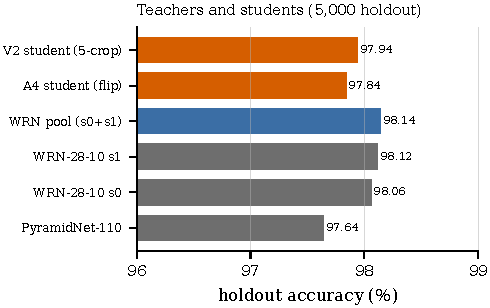
\includegraphics[width=\columnwidth]{figures/fig_teacher_student.pdf}
\caption{Teacher and student holdout accuracy. The 4.88M student is below the
best teacher pool but above the 28.5M PyramidNet teacher. A4 uses flip TTA and
V2 uses 5-crop, so the two student bars are not a controlled TTA comparison.}
\label{fig:teachers}
\end{figure}

\begin{table*}[t]
\centering
\small
\setlength{\tabcolsep}{4pt}
\caption{Main results on the fixed 5,000-image holdout and the leaderboard.
``Val'' is the best reported validation accuracy (raw for baseline, EMA for
KD/A4/V2, EMA+flip TTA for all tricks); ``5-crop'' is the 10-view TTA described
in Section~\ref{sec:setup}. Full-data models are trained on all 50k images and
have no honest validation score. The private 0.880 is the team's best of the two
selected submissions; both were selected, so the private 0.880 (13th) is not
attributed to a single row.}
\label{tab:main}
\begin{tabular}{@{}lcccccc@{}}
\toprule
Run & Architecture & Params & Epochs & Val & 5-crop & Public / Private \\
\midrule
Baseline & \texttt{r3\_64\_3-5-3} & 4.92M & 200 & 94.76 & -- & -- \\
All tricks, no KD & \texttt{r3\_64\_3-5-3} & 4.92M & 300 & 97.36 & -- & -- \\
KD, 2 teachers & \texttt{r3\_64\_3-5-3} & 4.92M & 600 & 97.74 & -- & 0.904 / -- \\
KD, 3 teachers & \texttt{r3\_64\_3-5-3} & 4.92M & 600 & 97.76 & -- & -- \\
A4 (3 teachers) & \texttt{r3\_80\_2-3-3} & 4.88M & 600 & 97.84 & 97.92 & -- \\
V2 (3 teachers) & \texttt{r3\_80\_2-3-3} & 4.88M & 1200 & 97.82 & 97.94 & -- \\
F1 / F2 (full data) & \texttt{r3\_80\_2-3-3} & 4.88M & 1200 & -- & -- & 0.898 / 0.899 \\
\textbf{F2s1 (selected)} & \texttt{r3\_80\_2-3-3} & 4.88M & 1200 & -- & -- & \textbf{0.911 / --} \\
\bottomrule
\end{tabular}
\end{table*}

\subsection{Architecture and Distillation Ablations}

At 300 epochs and with three teachers, the architecture sweep gives 97.38\% for
\texttt{r3\_64}, 97.42\% for \texttt{r3\_96}, and 97.62\% for \texttt{r3\_80}
(Figure~\ref{fig:curves}(b)). The wider first stage is worth about 0.24 points
over the baseline shape; the deeper/narrower alternative does not help. We
therefore use \texttt{r3\_80} for the main runs. The remaining two presets
(\texttt{r4\_64} and \texttt{r3\_40}) crashed early and produced no usable curve.

The KD hyperparameter sweep is similarly flat. With \texttt{r3\_80} at 300
epochs, temperature 2 reaches 97.62\% and temperature 1 with $\alpha=1$ reaches
97.50\%, both no better than the $T=4$ baseline (97.62\%;
Figure~\ref{fig:curves}(c)). Two teachers reach 97.74\% and three reach 97.76\%
at 600 epochs; the third teacher adds 0.02 points, which is smaller than the seed
spread. We keep three teachers for the main runs because the cost is modest and
the ensemble is more stable, but we do not claim a real accuracy gain from the
third teacher.

\subsection{Robustness and Augmentation}

\paragraph{The 150-epoch pilot.}
Figure~\ref{fig:b3} compares six policies at the same cheap schedule (150
epochs, no SAM, no KD). The control (TrivialAugment) reaches 96.48\% clean TTA
and 84.32\% on the composite proxy. RandAugment (96.50/83.70) and
AutoAugment-CIFAR (96.62/83.14) are slightly better on clean data and worse on
the proxy. Geometry-only (95.98/84.96) loses 0.50 clean for 0.64 proxy.
Affine+color (95.46/84.38) loses clean accuracy without a proxy gain. One-view
AugMix is the only policy that is clean-neutral (96.52, +0.04) and substantially
better on the proxy (87.42, +3.10). The pilot motivated the full 300-epoch test,
but its effect size is inflated: the 300-epoch control also improves a lot.

\begin{figure}[t]
\centering
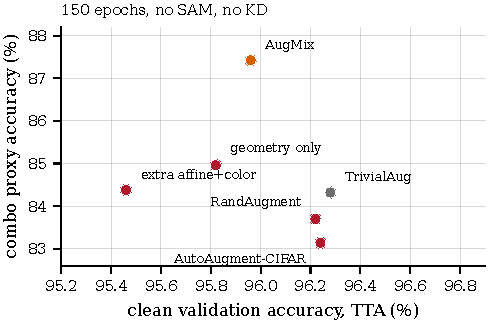
\includegraphics[width=\columnwidth]{figures/fig_b3_pilot.pdf}
\caption{Augmentation pilot at 150 epochs (no SAM, no KD). Each point is one
policy; the vertical axis is the composite corruption proxy. One-view AugMix is
the only policy that is clean-neutral and improves the proxy. The pilot
overstates the effect because the 300-epoch control is stronger.}
\label{fig:b3}
\end{figure}

\paragraph{The 300-epoch test.}
At 300 epochs with SAM, AugMix and the TrivialAugment control are identical on
clean validation (EMA 97.08\% both; flip TTA 97.04 vs.\ 97.22;
Figure~\ref{fig:robustness}). Under the no-TTA shifted evaluation, AugMix
improves the composite by 2.18 points (89.02 vs.\ 86.84, McNemar
$p=3.6\times10^{-9}$), Gaussian noise 0.05 by 4.30, and JPEG-30 by 5.16. Under
flip TTA it improves mild and strong photographic jitter by 1.10 and 1.38 points
($p\approx10^{-5}$). Geometry alone is where AugMix does nothing (+0.06 on
$\pm3$-pixel shifts), which is consistent with the gain coming from photometric
variation rather than framing. A second AugMix seed reproduces the effect (+1.80
composite; mean +1.99 across seeds) and keeps clean accuracy neutral (96.90\%).

\paragraph{Distillation.}
The provisional KD check uses the same \texttt{r3\_80} student, three teachers,
and 300 epochs, changing only \texttt{--autoaug}. In the checkpoint comparison at
epoch 200 of 300 (the archived logs stop earlier), AugMix is clean-neutral
($-0.12$, $p=0.56$) and better on the composite (+2.20,
$p=3.7\times10^{-12}$) and strong photographic jitter (+1.92,
$p=5.6\times10^{-12}$); the geometry proxy moves by +0.36 ($p=0.069$). At that
point the AugMix arm is level with the 600-epoch A4 model on the composite
(89.26 vs.\ 89.20) while still about one point behind on clean (96.86 vs.\
97.84). The effect therefore provisionally survives distillation at roughly the
same size as in the no-KD comparison. The run was interrupted and the two logs
stop at epochs 163 and 178 of 300; the comparison is provisional and was not used
for submission selection.

\paragraph{The JSD caveat.}
The B4/B5 variant is image-only, one-view AugMix without the Jensen-Shannon
consistency term. A separate 80-epoch AugMix+JSD finisher (JSD weight 12, ramped
over 10 epochs) behaved differently: it gained 2.2 points on the blur proxy
relative to the matched control but lost about one point on clean validation
(96.88 vs.\ 97.44 for the control and 97.84 for untouched A4). It failed our
clean-accuracy gate and was not submitted. The clean-neutral result should
therefore be read as specific to the one-view variant at the schedules we tested,
not to AugMix with JSD.

\begin{figure*}[t]
\centering
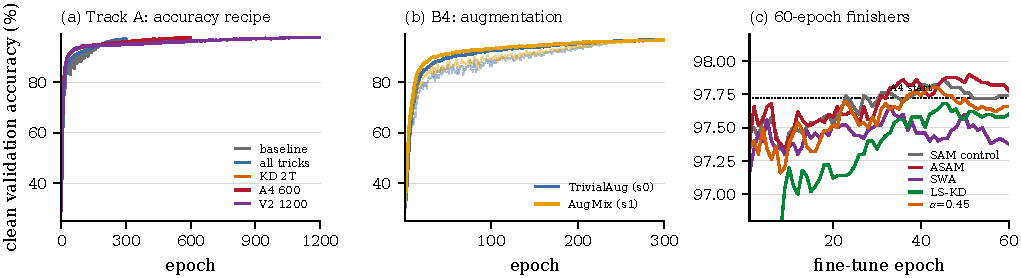
\includegraphics[width=\textwidth]{figures/fig_val_curves.pdf}
\caption{Validation curves (EMA weights unless noted, no TTA). (a) Main recipe:
baseline (raw), all tricks, two-teacher KD, A4 (600 epochs), and V2 (1,200
epochs). (b) Architecture sweep at 300 epochs. (c) KD-temperature/weight sweep;
the two logs stop at epochs 181 and 183 of 300. (d) 60-epoch continuations from
A4; the dotted line is the untouched A4 EMA on the same no-TTA evaluation
(97.72). The finishers stay within 0.35 points of it; none is a significant
gain. (e) Fresh 300-epoch alternatives: the WRN-40-2 pair, LS-KD, and fresh
ASAM; late training is shown and none beats the 97.66\% control. (f) The
provisional KD + AugMix arms; logs stop at epochs 163 and 178 of 300. Final
flip/5-crop TTA numbers are in Tables~\ref{tab:main} and~\ref{tab:negative}.}
\label{fig:curves}
\end{figure*}

\begin{figure*}[t]
\centering
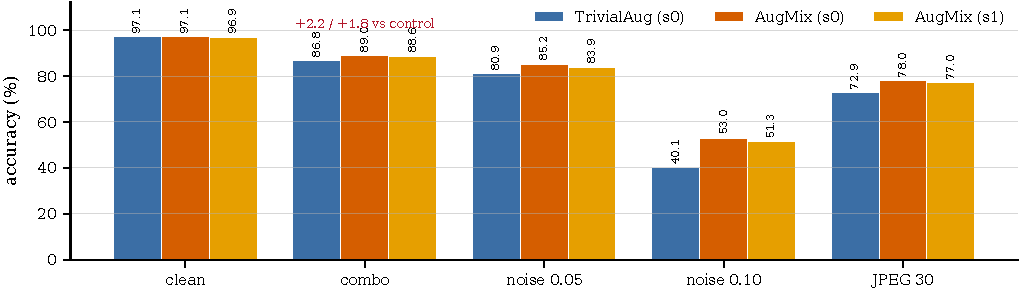
\includegraphics[width=\textwidth]{figures/fig_robustness.pdf}
\caption{Clean and shifted accuracy for the 300-epoch B4 arms (EMA weights, no
TTA). One-view AugMix is clean-neutral and improves the composite, noise, and
JPEG proxies; the two seeds give +2.18 and +1.80 on the composite. These are
label-free stress tests built from training images.}
\label{fig:robustness}
\end{figure*}

\subsection{Test-Time Augmentation}

Flip TTA is the default. The 10-view 5-crop procedure adds essentially nothing
on clean data (trivial $-0.02$, AugMix $+0.10$) and is a wash overall
(Figure~\ref{fig:tta}): it helps on JPEG and the composite by 0.5--1.2 points, but
loses on noise and zoom. It costs ten times the inference. We nevertheless used
5-crop for the 0.911 submission because it exactly reproduced the team's accepted
CSV; the gain over flip is inside leaderboard noise and should not be attributed
to TTA.

\begin{figure}[t]
\centering
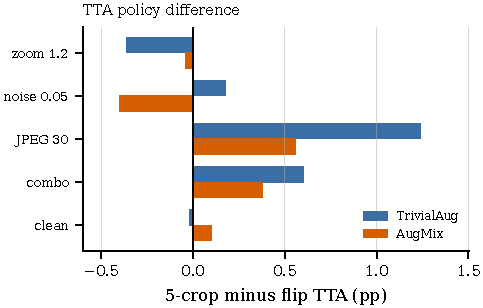
\includegraphics[width=\columnwidth]{figures/fig_tta_deltas.pdf}
\caption{5-crop minus flip TTA on the B4 arms. The multi-view policy helps on
JPEG and the composite, is negligible on clean data, and hurts on noise and zoom;
the 10$\times$ inference cost is not justified by the clean result.}
\label{fig:tta}
\end{figure}

\subsection{The Leaderboard}

Figure~\ref{fig:leaderboard} shows every public submission. The selected
\texttt{F2s1} 5-crop run is the best at 0.911; the two-teacher student is 0.904.
Late finishers and soups built on \texttt{F2s1} score 0.908, below the untouched
model, and test-time BN adaptation drops to 0.884. The private score is 0.880 and
the team finished 13th. The gap between the 97.94\% holdout and the 0.880 private
score is the central unexplained result: we do not have the final evaluation
labels or images, so we cannot identify whether it comes from a different capture
distribution, a harder class mix, or a smaller effective test set. We report it
as observed and do not tune against it.

\begin{figure}[t]
\centering
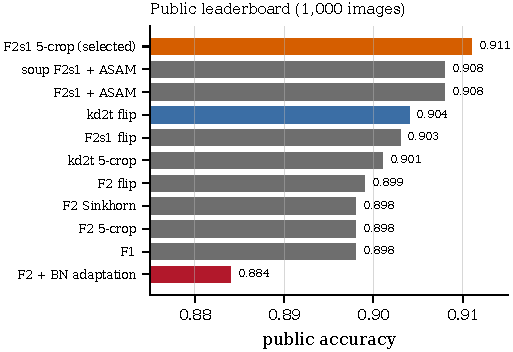
\includegraphics[width=\columnwidth]{figures/fig_leaderboard.pdf}
\caption{All public leaderboard submissions (1,000 images). The selected
\texttt{F2s1} 5-crop model is the best at 0.911; late ASAM/soup finishers sit at
0.908 and test-time BN adaptation at 0.884. Public scores carry roughly
$\pm1.1$pp of noise, so differences of a few images are not a model ranking.}
\label{fig:leaderboard}
\end{figure}

\section{What Did Not Work}
\label{sec:negative}

The competition rewarded clean accuracy, but a large fraction of our experiments
did not improve it. We report them here because the failure pattern is
informative: several techniques that are strong in the literature are neutral or
negative at this budget and schedule, and several apparent gains disappear under
a matched control. Table~\ref{tab:negative} summarizes the results; the text gives
the context.

\begin{table*}[t]
\centering
\footnotesize
\setlength{\tabcolsep}{2.5pt}
\caption{Techniques that did not pay off. $\Delta$ is in percentage points on the
5,000-image holdout unless the row uses the public leaderboard. Paired McNemar
$p$-values are shown where recorded; ``--'' means no paired test was logged.
Pilot numbers are clean TTA / combo; the B4 comparison is in
Table~\ref{tab:main}.}
\label{tab:negative}
\begin{tabular}{@{}p{0.17\textwidth}p{0.42\textwidth}rrp{0.17\textwidth}@{}}
\toprule
Technique & Matched comparison & $\Delta$ & $p$ & Verdict \\
\midrule
\multicolumn{5}{@{}l}{\emph{Augmentation (150-epoch pilot, clean TTA / combo)}}\\
RandAugment & 96.50 / 83.70 vs.\ 96.48 / 84.32 & $+0.02$ / $-0.62$ & -- & worse proxy \\
AutoAugment-CIFAR & 96.62 / 83.14 vs.\ control & $+0.14$ / $-1.18$ & -- & worse proxy \\
Geometry only & 95.98 / 84.96 vs.\ control & $-0.50$ / $+0.64$ & -- & clean drop \\
Extra affine+color & 95.46 / 84.38 vs.\ control & $-1.02$ / $+0.06$ & -- & clean drop \\
\midrule
\multicolumn{5}{@{}l}{\emph{Optimization and KD}}\\
ASAM continuation & 98.00 vs.\ 97.82 (SAM) & $+0.18$ & 0.049 & no gain over A4 \\
LS-KD (300 ep) & 97.62 vs.\ 97.62 (ordinary KD) & $0.00$ & -- & lower NLL only \\
WRN-40-2 pair & 97.26 vs.\ 97.62 (one \texttt{r3\_80}) & $-0.36$ & -- & loses \\
\midrule
\multicolumn{5}{@{}l}{\emph{Inference and adaptation}}\\
5-crop TTA & 97.20 vs.\ 97.22 (trivial); 97.16 vs.\ 97.06 (AugMix) & $-0.02$ / $+0.10$ & 1.0 / 0.33 & wash \\
Test-time BN & 0.884 vs.\ 0.899 public & $-1.5$ & -- & hurts \\
Sinkhorn balance & 0.898 vs.\ 0.899 public & $-0.1$ & -- & no gain \\
2-seed ensemble & +0.34 combo, +0.44 strong-photo & $+0.3$--$0.4$ & 0.15 / 0.02 & inside noise \\
Train-split BN & 97.08 / 97.20 vs.\ 97.92 / 97.94 & $-0.8$ / $-0.7$ & -- & hurts \\
\bottomrule
\end{tabular}
\end{table*}

\paragraph{Augmentation.}
RandAugment and AutoAugment-CIFAR are clean-neutral or slightly positive, but both
make the composite proxy worse than the TrivialAugment control. Geometry-only
augmentation trades 0.50 clean points for 0.64 proxy points, which fails our
clean-drop budget; affine+color loses 1.02 clean points with no proxy gain.
AugMix is the exception and is discussed in Section~\ref{sec:results}. The lesson
is that a policy can look competitive on clean validation and still be the wrong
choice for robustness; we therefore require both clean neutrality and a proxy
gain before adopting an augmentation.

\paragraph{ASAM and SWA.}
Figure~\ref{fig:curves}(c) shows the five 60-epoch continuations from A4; none
produces a significant gain over the untouched start. A 60-epoch ASAM continuation beats the matched SAM
continuation by 0.18 points (98.00 vs.\ 97.82, $p=0.049$), but it does not beat
the untouched A4 start point (97.92; $+0.08$, $p=0.50$). The confirm run from the
two-teacher student moves by +1 image against its SAM control and +2 against the
untouched model ($p=0.83$); pooled over both start points, ASAM versus the
untouched model is +6 of 10,000 images, but the two comparisons reuse the same
5,000 images, so this pooled count is exploratory. ASAM is better than SAM for
this late continuation, but the continuation itself does not improve the model.
SWA is neutral (97.80 vs.\ 97.82). A fresh 300-epoch ASAM run changes one image
(97.64 vs.\ 97.62); applying the 60-epoch ASAM finish to F2s1 changes 33/2,000
test labels and scores 0.908 public versus 0.911 for the untouched model; the
corresponding weight soup also scores 0.908. We did not launch fresh 1,200-epoch
ASAM/SWA runs.

\paragraph{LS-KD.}
Logit-standardized KD is a calibration intervention in our hands, not an accuracy
one. The continuation matches ordinary KD (97.76 vs.\ 97.82, within noise) and the
fresh 300-epoch run matches its ordinary-KD baseline exactly (97.62), while
substantially lowering validation NLL (0.086 vs.\ 0.154). If the metric rewarded
calibration, LS-KD would be attractive; for top-1 accuracy it is a wash.

\paragraph{Splitting the budget.}
Two WRN-40-2 models (2.24M each, 4.49M together) reach 97.10 and 97.08
individually; their equal-probability ensemble reaches 97.26. The ensemble gains
only +0.16 over one WRN and remains 0.36 below a single 4.88M \texttt{r3\_80}
(97.62). With this recipe, splitting the parameter budget into two smaller models
is worse than spending it on one. The pair's errors are also highly correlated
(111 images wrong in both; Jaccard overlap 0.61), so the ensemble has little
diversity to exploit.

\paragraph{TTA, adaptation, and ensembling.}
The 10-view TTA is a wash on clean data and only helps on JPEG/composite proxies;
flip TTA captures most of it. Test-time BN adaptation, which recomputes BN
statistics on the evaluation images, drops the public score from 0.899 to 0.884.
Sinkhorn class balancing is neutral (0.898 vs.\ 0.899). A two-seed AugMix
ensemble gains +0.34 on the composite ($p=0.15$) and +0.44 on strong photographic
jitter ($p=0.02$), but the composite gain is not significant and both are inside
the public-LB noise; we did not use an ensemble for the final submission.
Train-split BN recalibration (recomputing BN on clean training images) hurts
badly: 97.08 vs.\ 97.92 for A4 and 97.20 vs.\ 97.94 for V2. The saved BN
statistics are already well matched to the evaluation transform; replacing them
with clean-image statistics removes the augmentation-induced robustness.

\paragraph{Fresh 300-epoch sweep.}
A matched 300-epoch sweep found no gain from extra regularization or a different
KD weight: two-teacher KD is neutral (97.66), KD $\alpha=0.45$ loses 11 images,
and stochastic depth 0.1 loses 18 (97.30 vs.\ 97.66, $p=0.005$).

\paragraph{What we did not test.}
DKD, structural teacher pruning, SE blocks, and fresh 1,200-epoch ASAM/SWA/LS-KD
runs were left untested; they are the most promising follow-ups but did not fit
the compute budget.

\section{Full Run Log}
\label{sec:appendix}

Table~\ref{tab:runs} lists every run discussed in the paper with the numbers used
for the figures. All validation numbers use the fixed seed-0 5,000-image holdout;
``5-crop'' marks the 10-view TTA. Public scores are the Kaggle public leaderboard
(1,000 images) and are only reported for submitted models.

\begin{table*}[t]
\centering
\footnotesize
\setlength{\tabcolsep}{4pt}
\caption{Full run log. Val is EMA accuracy (flip TTA unless marked 5-crop);
public is the Kaggle public leaderboard. The first block is the main accuracy
path, the second is KD/architecture, the third is late finishers and failures.}
\label{tab:runs}
\begin{tabular}{@{}llcc@{}}
\toprule
Run & Setup & Val & Public \\
\midrule
\multicolumn{4}{@{}l}{\emph{Main accuracy path}}\\
Baseline & r3\_64, 200 ep, crop+flip & 94.76 & -- \\
All tricks & r3\_64, 300 ep, TA+Cutout+mix+SAM+EMA & 97.36 & -- \\
KD 2 teachers & r3\_64, 600 ep & 97.74 & 0.904 \\
KD 3 teachers & r3\_64, 600 ep & 97.76 & -- \\
A4 & r3\_80, 600 ep, 3 teachers & 97.84 / 97.92 (5-crop) & -- \\
V2 & r3\_80, 1200 ep, 3 teachers & 97.82 / 97.94 (5-crop) & -- \\
F2s1 & r3\_80, 1200 ep, full data, seed 1 & -- & 0.911 \\
\midrule
\multicolumn{4}{@{}l}{\emph{Architecture and KD ablations (300 ep)}}\\
r3\_64 sweep & 3/5/3, 4.92M & 97.38 & -- \\
r3\_80 sweep & 2/3/3, 4.88M & 97.62 & -- \\
r3\_96 sweep & 2/2/2, 4.90M & 97.42 & -- \\
A3 T=2 & r3\_80, KD temperature 2 & 97.62 & -- \\
A3 T=1, $\alpha$=1 & r3\_80, KD temperature 1 & 97.50 & -- \\
\midrule
\multicolumn{4}{@{}l}{\emph{Late finishers (60 ep from A4, 5-crop)}}\\
SAM control & C60\_sam & 97.82 & -- \\
ASAM & C60\_asam & 98.00 & -- \\
KD $\alpha$=0.45 & C60\_a045 & 97.96 & -- \\
LS-KD & C60\_lskd & 97.76 & -- \\
SWA & C60\_swa & 97.80 & -- \\
\midrule
\multicolumn{4}{@{}l}{\emph{Fresh alternatives and failures}}\\
Fresh ASAM & S300\_asam, 300 ep & 97.64 & -- \\
Fresh LS-KD & F300\_lskd, 300 ep & 97.62 (5-crop) & -- \\
WRN-40-2 s0 & 2.24M, 300 ep & 97.10 & -- \\
WRN-40-2 s1 & 2.24M, 300 ep & 97.06 & -- \\
WRN pair & equal-probability average, 4.49M total & 97.26 & -- \\
J80 control & 80-ep AugMix control & 97.44 & -- \\
J80 JSD & 80-ep AugMix+JSD & 96.88 & -- \\
Test-time BN & F2, BN recomputed on test & 97.34 & 0.884 \\
Sinkhorn & F2, class-balanced prediction & -- & 0.898 \\
5-crop TTA & B4 trivial / AugMix & 97.20 / 97.16 & -- \\
\bottomrule
\end{tabular}
\end{table*}

\section{Discussion and Limitations}
\label{sec:discussion}

\paragraph{What produced the accuracy.}
The largest single jump came from the training recipe rather than the
architecture: the baseline at 94.76\% became 97.36\% with long training,
TrivialAugment, Cutout, mixup/CutMix, SAM, and EMA. KD added another 0.4 points,
and the wider student added about 0.2. The 4.88M student ends up better than the
28.5M PyramidNet teacher and within 0.3 points of the best teacher pool. This is
consistent with the view that a long, well-regularized student can absorb the
teacher ensemble's function without inheriting its capacity. Architecture search
inside the 5M budget was secondary: the best shape is only 0.24 points above the
baseline shape at 300 epochs.

\paragraph{The unexplained gap.}
Our best holdout number is 97.94\% (5-crop); the selected submissions scored
0.911 and 0.904 public, and the team's private score was 0.880. The private score
is roughly ten points below the holdout number, and the gap between the best
public score (0.911) and the private score (0.880) is 3.1 points. The
public/private split is 1,000 images each, so part of the 3.1-point difference is
sampling noise; the rest could be a harder private subset, a different capture
distribution, or both. We do not have the final evaluation images or labels, so
we cannot separate these causes. The gap is reported as observed, not as
something the method was tuned to fix.

\paragraph{Why one-view AugMix was not shipped.}
One-view AugMix is the one robustness intervention that survived every check we
ran: it is clean-neutral at 300 epochs, improves the composite by 2.2 points,
improves photographic jitter by 1.1--1.9 points, replicates across seeds, and
keeps its effect under three-teacher KD. It was still not in the final submission.
The KD confirmation finished after the team had selected its submissions; its logs
stop at epoch 178/300, and the full-data 1,200-epoch AugMix run was never trained.
Given that the final private gap is unexplained, we cannot claim that shipping
AugMix would have improved the score. The honest conclusion is that it was the
best-supported robustness candidate we had, and the submission schedule did not
allow us to test it at the shipping scale.

\paragraph{Limitations.}
Most comparisons use a single seed; the exceptions are the two AugMix seeds and
the ASAM confirm. The holdout is 5,000 images, so the seed-to-seed spread is
0.2--0.4 points and small differences should not be over-interpreted. The B5 KD
comparison is provisional at 200/300 epochs and was interrupted twice; its
partial curves are in Figure~\ref{fig:curves}(f). The corruption and
photographic proxies are synthetic and label-free; they are stress tests, not
models of the final shift. The public and private leaderboards are 1,000 images
each, so the leaderboard itself is noisy. We did not run fresh 1,200-epoch ASAM,
SWA, or LS-KD experiments, and we did not test DKD or structural teacher pruning.
Finally, the full-data models have no unbiased validation score, so the final
selection relies on the holdout models and the team's judgment.

\paragraph{What we would do differently.}
First, ablate augmentation at the shipping schedule, not at a cheap pilot: the
150-epoch pilot overstated AugMix's effect because the 300-epoch control improved
so much. Second, keep per-epoch logs for every run in the repository; several
curves in this paper are missing because the logs stayed on a cluster or a cloud
volume. Third, complete the KD robustness run before submission selection, so
that a clean-neutral augmentation has a chance to ship. Fourth, treat the public
leaderboard as a noisy estimate and select by paired holdout comparisons, which
is what the team did. Fifth, run the main comparisons with at least two seeds;
the single-seed spread is large enough to swallow several of the effects we
measured.

\section{Conclusion}
\label{sec:conclusion}

We trained a 4.88M-parameter ResNet from scratch on CIFAR-10 and reached 97.84\%
clean validation accuracy (97.92\% with 10-view TTA). The team's selected
submissions scored 0.911 and 0.904 public, with a private score of 0.880 and
13th place. The
recipe is ordinary in its ingredients---long cosine training, SAM, EMA,
TrivialAugment, Cutout, mixup/CutMix, and three-teacher KD---but the combination
is strong at this parameter budget, and the student beats its largest teacher.

The project also produced a useful catalog of negative results. RandAugment,
AutoAugment-CIFAR, geometry-only and affine+color augmentation, ASAM/SWA
fine-tuning, logit-standardized KD, a two-model parameter split, multi-crop TTA,
test-time BN adaptation, Sinkhorn balancing, and seed ensembling all failed to
improve the metric in our hands. One-view AugMix was the exception: clean-neutral and
consistently better on corrupted and photometric proxies, but not shipped because
its KD confirmation finished after submission selection.

The unresolved question is the roughly ten-point gap between clean validation and
the private leaderboard. We do not have the final evaluation images or labels,
so we can describe the gap but not explain it. We hope the
negative results and the explicit separation between proxy evidence and
leaderboard evidence are useful to others working under similar constraints.

\paragraph{Reproducibility.}
Every run writes \texttt{args.json}, a per-epoch \texttt{log.csv}, a
\texttt{results.json}, and a resumable \texttt{last.pt}. The report folder
contains the archived logs, the fixed figure-generation script, and the AAAI
style file; every figure can be rebuilt without the competition data or any
checkpoint. The submitted models are 4.88M and 4.92M parameters, trained from
scratch with no external data.


\end{document}
